%Paul E. West

%\documentclass[xcolor=svgnames]{beamer}
\documentclass{beamer}
\usepackage[boxed,vlined,figure]{algorithm2e}

%\usecolortheme[named=FireBrick]{structure}
%\usecolortheme[named=black]{structure}
%\usecolortheme{beetle}
%\usecolortheme{beaver}
%\usecolortheme{crane}
%\usecolortheme{dolphin}
%\usecolortheme{dove}
%\usecolortheme{fly}
%\usecolortheme{lily}
\usecolortheme{orchid}
%\usecolortheme{rose}
%\setbeamercolor{background canvas}{bg=Gold!25}
%\setbeamercolor{background canvas}{bg=Black!100}
%\setbeamercolor{foreground}{bg=Gold!25}
%\setbeamercolor{normal text}{fg=green,bg=black}
%\setbeamercolor*{palette primary}{use=structure,fg=green,bg=black}

\mode<presentation>{
    \usetheme{Darmstadt}
    \setbeamercovered{invisible}
    %\setbeamercovered{transparent}
    \setbeamercolor*{palette primary}{use=structure,fg=white,bg=blue}
    \setbeamercolor*{palette secondary}{use=structure,fg=white,bg=blue}
    \setbeamercolor*{palette tertiary}{use=structure,fg=white,bg=blue}
}

\usepackage[english]{babel}
\usepackage[latin1]{inputenc}
\usepackage{times}
\usepackage[T1]{fontenc}
%\usepackage{epsfig}
\usepackage{ulem}
\usepackage{color,soul}

\usepackage{graphicx}
\usepackage{amssymb}
\usepackage{url,hyperref}
\definecolor{beamer@blendedblue}{rgb}{1,.6,.2}
%\usepackage{tikz}
%\usetikzlibrary{shapes}
%\usetikzlibrary{arrows}
%\tikzstyle{block}=[draw opacity=0.7, line width=1.4cm]
\usepackage{listings}
\lstset{language=Java}
\lstset{showspaces=false}
\lstset{showstringspaces=false}
\lstset{tabsize=4}
\lstset{basicstyle=\tiny}


%\usecolortheme[overlystylish]{albatross}
%\usecolortheme[]{lily}
%\usecolortheme[]{albatross}
%\usecolortheme[]{orchid}
%\setbeamercolor{normal text}{fg=green!10}

\title{COIN 315: Data Structures}
\author{Dr. Paul E. West}

\institute{
  Department of Computer Science\\
  Charleston Southern University
}

\date{August 24, 2015}

\subject{Software Programming}
%\keywords{Performance Counters, Multicore}

%\pgfdeclareimage[height=1.0cm]{university-logo}{../imgs/csu-logo}
\pgfdeclareimage[height=0.75cm]{university-logo}{../imgs/csu-logo}
%\pgfdeclareimage[height=0.50cm]{university-logo}{../imgs/csu-logo}
\logo{\pgfuseimage{university-logo}}

\begin{document}

\begin{frame}
  \titlepage
\end{frame}

\section{Introduction}
\subsection{}
\begin{frame}{About the Professor}
\begin{itemize}
\item PhD from Florida State University in Computer Science
\item Faculty Experience:
\begin{itemize}
\item Charleston Southern: Assistant 2015-Present
\item College of Charleston: Adjunct 2013-2014
\end{itemize}
\item Work Experience:
\begin{itemize}
\item Google (2014): Android Bluetooth/Wi-Fi/Telephony
\item SPAWAR (2009-2014, 2015): Communication systems
\item Various Government Contracts: (2016 - Present)
\item DenimGroup (2004-2005): Start-up; web design and network security
\end{itemize}
\end{itemize}
\end{frame}

\begin{frame}{What is a Data Structure?}
\begin{columns}[c]
\column{0.50\textwidth}
\begin{itemize}
\item A data structure is a scheme for organizing data in the memory of a computer. 
\item Some of the more commonly used data structures include lists, arrays, stacks, queues, heaps, trees, and graphs.
\end{itemize}
\column{0.50\textwidth}
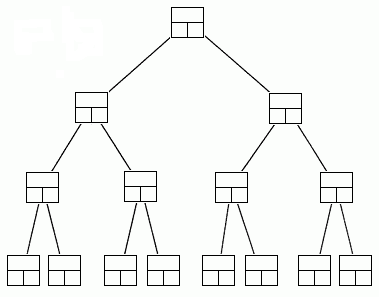
\includegraphics[width=1.0\textwidth]{../imgs/binary-tree.png}
\end{columns}
\end{frame}

\begin{frame}{Why?}
\begin{columns}[c]
\column{0.50\textwidth}
\begin{itemize}
\item The way in which the data is organized affects the performance of a program for different tasks. 
\item Computer programmers decide which data structures to use based on the nature of the data and the processes that need to be performed on that data.
\end{itemize}
\column{0.50\textwidth}
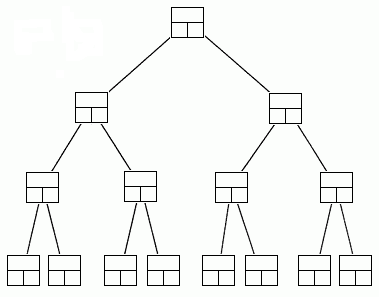
\includegraphics[width=1.0\textwidth]{../imgs/binary-tree.png}
\end{columns}
\end{frame}

\begin{frame} {Queue}
\begin{itemize}
\item A queue is an example of commonly used simple data structure.  A queue has beginning and end, called the front and back of the queue. 
\end{itemize}
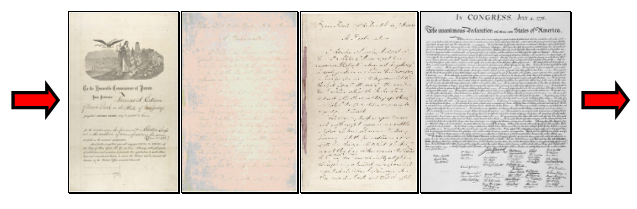
\includegraphics[width=1.0\textwidth]{../imgs/queue.png}
\begin{itemize}
\item Data enters the queue at one end and leaves at the other. Because of this, data exits the queue in the same order in which it enters the queue, like people in a checkout line at a supermarket.
\end{itemize}
\end{frame}

\begin{frame}{Binary Trees}
\begin{columns}[c]
\column{0.50\textwidth}
\begin{itemize}
\item A binary tree is another commonly used data structure. It is organized like an upside down tree. 
\item Each spot on the tree, called a node, holds an item of data along with a left pointer and a right pointer. 
\end{itemize}
\column{0.50\textwidth}
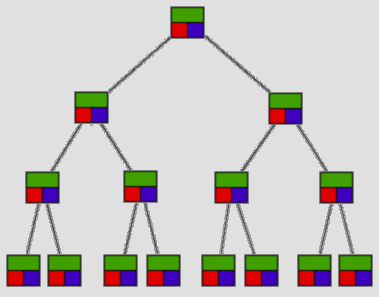
\includegraphics[width=1.0\textwidth]{../imgs/binary-tree-color.png}
\end{columns}
\end{frame}

\begin{frame}{Binary Trees}
\begin{columns}[c]
\column{0.50\textwidth}
\begin{itemize}
\item The pointers are lined up so that the structure forms the upside down tree, with a single node at the top, called the root node, and branches increasing on the left and right as you go down the tree.
\end{itemize}
\column{0.50\textwidth}
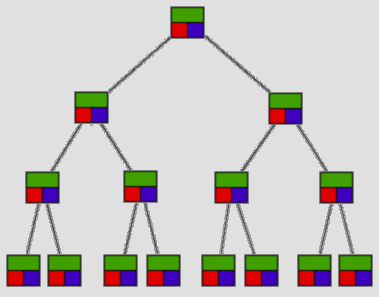
\includegraphics[width=1.0\textwidth]{../imgs/binary-tree-color.png}
\end{columns}
\end{frame}

\begin{frame}{Decisions Decisions...}
\begin{columns}[c]
\column{0.50\textwidth}
\begin{itemize}
\item When do we choose one over the other?
\end{itemize}
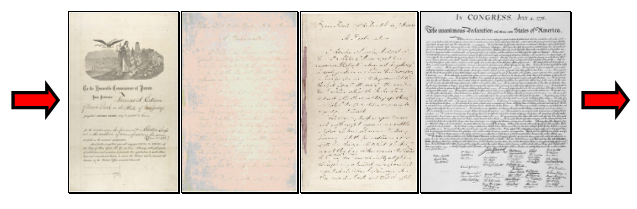
\includegraphics[width=1.0\textwidth]{../imgs/queue.png}
\column{0.50\textwidth}
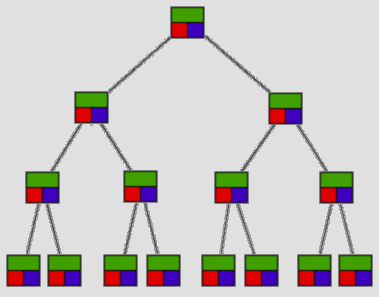
\includegraphics[width=1.0\textwidth]{../imgs/binary-tree-color.png}
\end{columns}
\end{frame}

\section{Syllabus}
\subsection{}

\begin{frame}{Syllabus}
Lets go over the syllabus...
\end{frame}

\begin{frame}{Warning:}
\begin{itemize}
\item Most students consider this class high(est) workload
\item This class really prepares your for work experience
\end{itemize}
\end{frame}

\begin{frame}{Do Not Drop!}
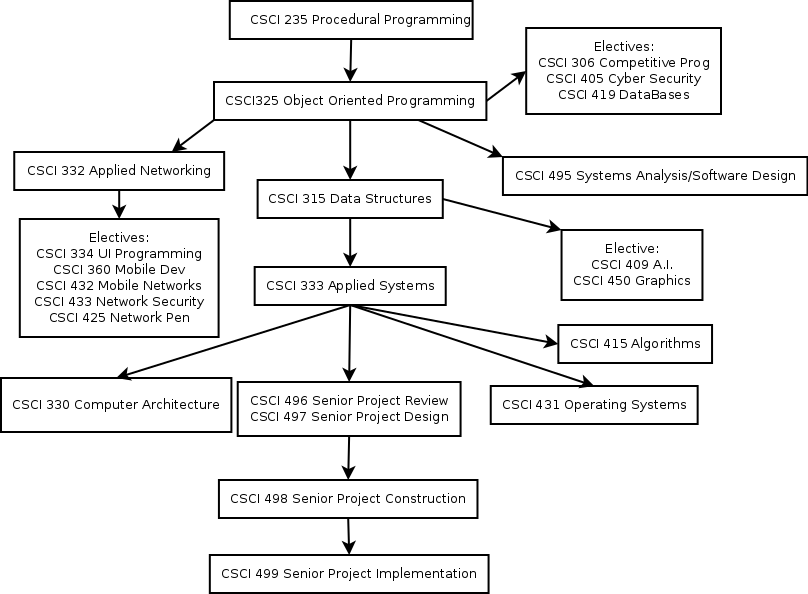
\includegraphics[width=0.8\textwidth]{../imgs/cs-major.png}
\end{frame}

\section{Tools}
\subsection{}
\begin{frame}{}
\begin{itemize}
\item git: used as our repository of code, lectures, and assignments
\item gcc: a compiler toolchain used to translate our C++ programs into machrine executable programs
\item cxxtest: a test suite to build and automate are testing
\item make: a tool to simplify building, testing, cleaning, and other utilities
\item text editor: use to write your programs
\item bash: our shell/Command Line Interface we use to run our programs
\item These tools make up our development environment
\item How is this different than an IDE?
\end{itemize}
\end{frame}

\begin{frame}{Logging into our machines}
\begin{itemize}
\item Our lab uses Linux (Debian 8)
\item Please login with your standard CSCI login
\item \textbf{\textit{Note:}} These installations of Debian has different GUIs to utilize, you may choose your preference by clicking on the gear when entering your password!
\begin{itemize}
\item I recommend starting with KDE or Gnome.
\item I personally use Enlightenment.
\end{itemize}
\item You may run Linux at home natively or as a VM, I recommend Mint or Ubuntu if you are new.
\end{itemize}
\end{frame}

\begin{frame}{Terminal}
\begin{itemize}
\item terminal: (terminal emulator), is a text-only window in a graphical user interface (GUI) that emulates a console. 
\item It is were we use our CLI
\item xterm, gterminal, lxdeterminal
\item Run whatever you want!
\end{itemize}
\end{frame}

\section{Terminal}
\subsection{}

\begin{frame}{UNIX Command Format}
\begin{itemize}
\item UNIX commands can be very simple one word commands, or they can take a number of additional arguments (parameters) as part of the command. In general, a UNIX command has the following form: \\
\textbf{command} options(s) filename(s)
\item The command is the name of the utility or program that we are going to execute. 
\item The options modify the way the command works. It is typical for these options to have be a hyphen followed by a single character, such as -a. It is also a common convention under Linux to have options that are in the form of 2 hyphens followed by a word or hyphenated words, such as --color or --pretty-print. 
\item The filename is the last argument for a lot of UNIX commands. It is simply the file or files that you want the command to work on.
\end{itemize}
\end{frame}

\begin{frame}{Common UNIX Conventions}
\begin{itemize}
\item In UNIX, the command is almost always entered in all lowercase characters. 
\item Typically any options come before filenames.
\item Many times, individual options may need a word after them to designate some additional meaning to the command.
\end{itemize}
\end{frame}

\begin{frame}{Man Page}
\begin{itemize}
\item The man command allows you to access the MANual pages for a UNIX command.
\item To get additional help on any of the commands listed below, you can always type man name\_of\_command at the command prompt.
\item Examples:\\
man ls \\
man cd
\end{itemize}
\end{frame}


\begin{frame}{Navigation and Directories}
\begin{itemize}
\item ls: lists the contents of a directory
\begin{itemize}
\item l: long directory listing
\item a: lists all files, including files which are normally hidden
\item F: distinguishes between directories and regular files
\item h: ?  Look it up using man
\end{itemize}
\item pwd: prints the current working directory
\item cd: changes directories
\begin{itemize}
\item The difference between relative and absolute paths.
\item Special characters ., .., and ~.
\end{itemize}
\item mkdir: creates a directory
\item rmdir: removes a directory (assuming it is empty)
\item If you get an error that the directory is not empty even though it looks empty, check for hidden files.
\end{itemize}
\end{frame}

\begin{frame}{Commands}
\begin{itemize}
\item cat : shows the contents of a file, all at once
\item more : shows the contents of a file, screen by screen
\item less : also shows the contents of a file, screen by screen
\item head : used to show so many lines form the top of a file
\item tail : used to show so many lines form the bottom of a file
\end{itemize}
\end{frame}

\begin{frame}{Commands}
\begin{itemize}
\item alias: creates an alias for a command.
\begin{itemize}
\item Aliases can be placed in your ~/.bashrc login script.
\item Example: alias rm 'rm -i'.
\end{itemize}
\item date: shows the date and time on the current system
\item who: used to print out a list of users on the current system
\item hostname: prints the hostname of the current computer
\item whoami: prints your current username
\end{itemize}
\end{frame}

\begin{frame}{Commands}
\begin{itemize}
\item The pipe (|) creates a channel from one command to another. Think of the pipe as a way of connecting the output from one command to the input of another command.
\item The pipe can be used to link commands together to perform more complex tasks that would otherwise take multiple steps (and possibly writing information to disk).
\item Examples:
\begin{itemize}
\item Count the number of users logged onto the current system.
\begin{itemize}
\item The who command will give us line by line output of all the current users.
\item We could then use the wc -l to count the number of lines...
\item who | wc -l
\end{itemize}
\item Display long listings in a scrollable page.
\begin{itemize}
\item ls | less
\end{itemize}
\end{itemize}
\end{itemize}
\end{frame}

\begin{frame}{Commands}
\begin{itemize}
\item ps : lists the processes running on the machine. 
\begin{itemize}
\item ps -u username lists only your processes. 
\item ps -a : lists all processes running on the machine.
\item The PID column of the listing, provides the information required by the kill command.
\end{itemize}
\item kill : terminates a process
\begin{itemize}
\item kill process\_id : sends a terminate signal to the process specified by the process\_id (PID).
\item In cases where the terminate signal does not work, the command ``kill -9 process\_id" sends a kill signal to the process.
\end{itemize}
\item nice : runs a process with a lower priority.
\end{itemize}
\end{frame}

\section{Weapons}
\subsection{}

\begin{frame}{Editor War!}
\begin{itemize}
\item vi: (vee-eye) large learning curve, but can increase productivity
\item emacs: has numerous features and more beginner friendly
\item ``standard editors:''
\begin{itemize}
\item kate
\item gedit
\item tea
\item jed
\end{itemize}
\item to exit vim: pres ESC : x $<$enter$>$
\item to exit emacs: ctrl-x, ctrl-c
\item I recommend starting with a standard one and then branching out.
\item I use vi
\end{itemize}
\end{frame}

\subsection{}
\begin{frame}{Git}
\begin{itemize}
\item Developed by Linus Torvalds
\item Version Control Tool
\begin{itemize}
\item Subversion
\item CVS
\end{itemize}
\item Open Source 
\item Free!
\item Just a folder in a directory
\end{itemize}
\end{frame}

\begin{frame}{Git Golden 5}
\begin{itemize}
\item clone/init
\item Add
\item Commit
\item Push
\item Pull
\end{itemize}
\end{frame}

\begin{frame}{Joining the Class}
\begin{itemize}
\item Create a GitHub account (or use an existing one) and login.
\item email me you username: pwest@csuniv.edu
\item You should (eventually) receive an email to join CSU
\item Click the link and join
\item Click on the csci-315-fall-2015 repository
\item Click fork
\item Now clone your repository:\\
\$ git clone $<$your repo$>$
\item Lets look through the repository...
\end{itemize}
\end{frame}

\section{Lab Assignment 0}
\subsection{}
\begin{frame}{}
\begin{itemize}
\item Follow the instructions for Lab 0
\end{itemize}
\end{frame}

%\begin{frame}{Event Based Processor}
%\begin{columns}[c]
%\column{0.25\textwidth}
%\begin{block}{OS driven Execution}
    %\includegraphics[width=1.0\textwidth]{imgs/normproc.png}
%\end{block}
%\column{0.25\textwidth}
%\begin{block}{Event Driven Execution}
    %\includegraphics[width=1.0\textwidth]{diagrams/eventproc.png}
%\end{block}
%\column{0.5\textwidth}
%\begin{itemize}
    %\item Normal execution: kernel/software driven
    %\item Event based : event driven
    %\item Performance monitoring is event based
    %\item Next task based on event not scheduled by kernel
    %\item 5.92 times speedup for control dominated programs
%\end{itemize}
%\end{columns}
%\end{frame}

\end{document}
